%% START EDUCATION CHAPTER
\chapter{\educationtitle}
\label{chap:education}
\clearpage

With rapid advances in sequencing technologies, the entire field of biology has largely shifted to depend upon the ability to analyze ultra-large datasets. As a result, the ability to perform basic computation has become a necessary prerequisite to successful biological research, yet it is only barely beginning to enter official undergraduate biology curricula as a required topic. Further, these skills are required by not only undergraduate biologists, but by graduate students, post-docs, and even faculty members and professionals, yet these individuals may not have the ability to enroll in undergraduate Computer Science courses. In an attempt to address this gap in education availability, I have dedicated significant effort to develop \glspl{MAIT} for use in \glspl{MOOC} as well as in flipped in-person classrooms.

\section{Introduction}
\subsection{Bioinformatics Education: The New Frontier}
With the introduction of \gls{NGS} technologies, researchers gained the ability to perform large-scale sequencing experiments at extremely high throughput with relatively low costs~\cite{Metzker2010}. Due to the massive size of the datasets that are produced in such experiments, basic computational education has become increasingly necessary for successful biological research. While professors at top universities have started introducing bioinformatics courses into undergraduate curricula in recent years~\cite{Compeau2019,Mulder2018,Madlung2018}, access to such courses is typically restricted to students who have the ability to \textit{enroll} in undergraduate courses at these top universities. However, high tuition costs disproportionately prevent low-income and minority students from entering such universities~\cite{Wetzel1998}, leading to disparity in terms of who actually has access to such learning materials. Further, due to the rapidly growing popularity of computational courses~\cite{Camp2017}, instructors of such courses tend to struggle to scale their courses to accommodate large class sizes.

\subsection{The MOOC Revolution}
With the creation of companies like Coursera and edX, university professors started to develop \glspl{MOOC}: tuition-free courses taught over the internet to a large number of students. What started with just a handful of courses, such as \textit{Machine Learning} by Andrew Ng (2012)~\cite{Ng2012}, eventually blew up, and all major universities had started releasing \glspl{MOOC} on a wide range of subjects~\cite{Pappano2012}. Much research went into how to design these courses~\cite{Guardia2013,Bruff2013,Breslow2013,Guo2014}, but their reception was generally mixed: some enjoyed the freedom of filling their education gaps at their own pace~\cite{Milligan2017}, whereas others were pessimistic about their educational value~\cite{Vardi2012}. Many complaints were with regard to the passive learning encompassed in traditional \glspl{MOOC}, in which students simply watch a series of lecture videos and answer simple multiple choice quizzes embedded throughout.

\subsection{From MOOCs to MAITs}
In 2014, Phillip Compeau and Pavel Pevzner released the first ever bioinformatics \gls{MOOC}, \textit{Bioinformatics Algorithms}~\cite{Compeau2014}, and with it, a new technology to revolutionize online learning: the \gls{MAIT}, an online text that has integrated quizzes, numerical problems, and even coding challenges to allow the learner to directly interact with the content and to allow the instructor to enable active learning, even in a remote and automated setting~\cite{Compeau2015}. The challenges are adaptive in that they provide the student uniquely-tailored feedback based on the student's specific misconception, and the text itself is adaptive in that the user can take his or her own unique ``learning path.'' For example, a biology student would have the ability to take optional ``detours'' on prerequisite computer science topics such as time complexity, whereas a computer science student would have the ability to take optional ``detours'' on prerequisite biology topics such as the Central Dogma. These carefully-written \glspl{MAIT} were the foundation upon which the \textit{Bioinformatics Algorithms} \glspl{MOOC} were built, and the adaptivity and interactivity was generally well-received by the learners.

\subsection{``Bioinformatics'' Means Nobody Gets Left Behind}
Despite the great success of the \textit{Bioinformatics Algorithms} \glspl{MOOC}, the space of online bioinformatics education was not yet filled: these courses were excellent for students with extensive backgrounds in programming, discrete mathematics, and algorithms, but for all biologists who wanted to transition into the computational aspects of the field, these courses were incomprehensible due to the students' lack of computational background. This motivated my work in bioinformatics education: the development of beginner-friendly \glspl{MAIT} to embed within \glspl{MOOC} as well as to integrate into offline classrooms.

\section{Methods}
\subsection{Teaching Philosophy}
Just like running a traditional offline classroom, developing a \gls{MAIT} requires the implementation of various pedagogical techniques to optimize the learning experience and to enhance student outcomes. As such, the pedagogical design of a \gls{MAIT} is essential to its success.

\subsubsection{Bloom's Taxonomy}
Bloom's Taxonomy is a set of three hierarchical models used to classify educational learning objectives into levels of complexity and specificity~\cite{Bloom1956}. The cognitive (i.e., knowledge-based) domain of the taxonomy is a hierarchy containing the following levels: Remember, Understand, Apply, Analyze, Evaluate, and Create (Fig.~\ref{fig:education-bloom-taxonomy})~\cite{Anderson2001}. I followed the guidelines of Bloom's Taxonomy in developing my materials.

\begin{figure}
\centering
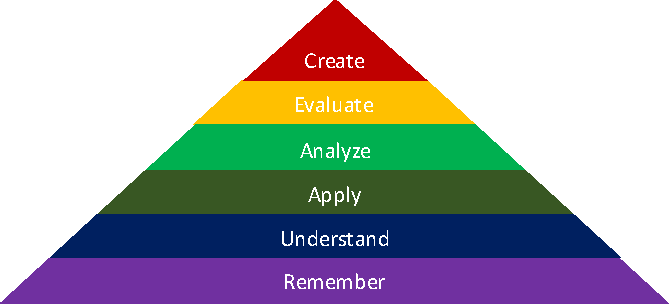
\includegraphics[width=0.65\textwidth]{figs/education-bloom-taxonomy}
\caption[Bloom's Taxonomy]
{Bloom's Taxonomy}
\label{fig:education-bloom-taxonomy}
\end{figure}

\subsubsection{Active Learning}
Within my \glspl{MAIT}, I implement the Active Learning approach~\cite{Bonwell1991}: students actively engage with the materials as opposed to simply passively reading or viewing them. Specifically, I integrate numerous multiple choice, short answer, numerical, and coding challenges that can be solved directly within the text. All challenges are automatically graded via carefully-designed \glspl{ITS}, which attempt to provide the student personalized feedback based on the student's unique misconceptions (Fig.~\ref{fig:education-code-challenge}).

\begin{figure}
\centering
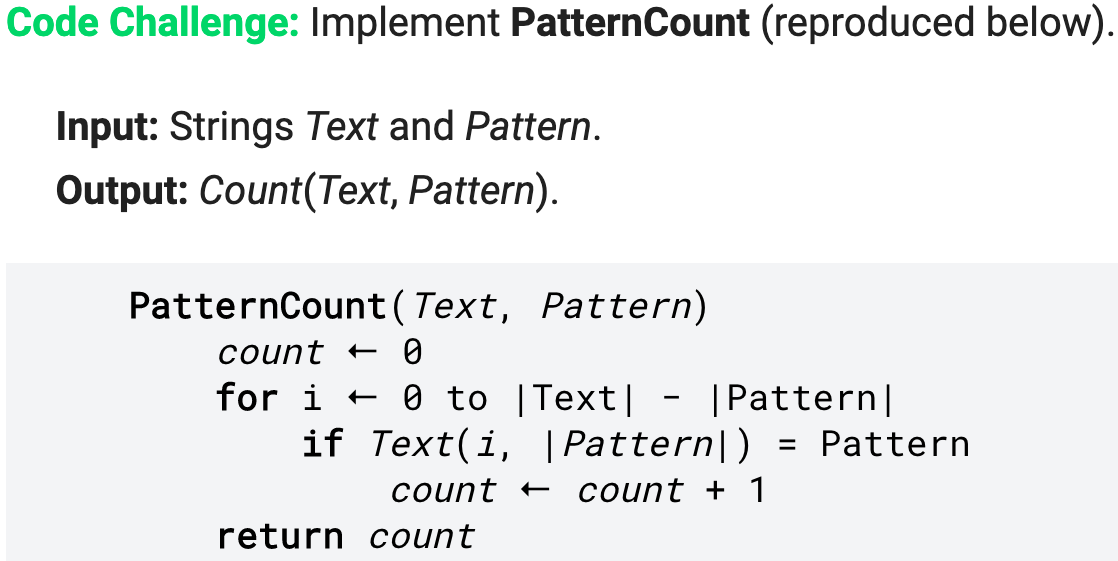
\includegraphics[width=0.85\textwidth]{figs/education-code-challenge-prompt}\\
(a)\\
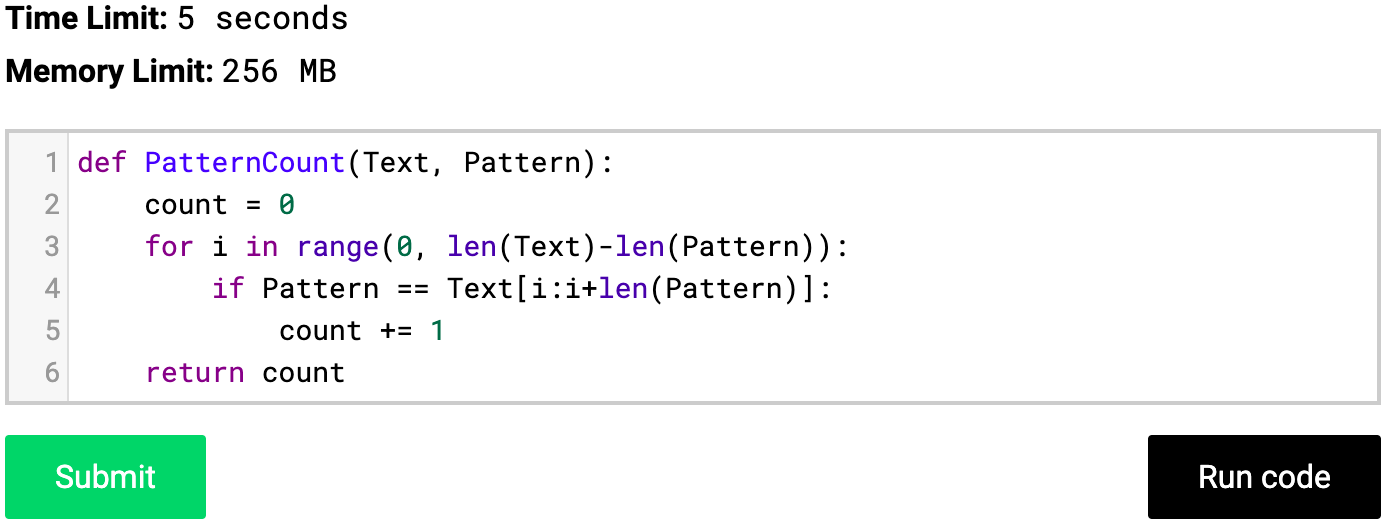
\includegraphics[width=0.85\textwidth]{figs/education-code-challenge-bug}\\
(b)\\~\\
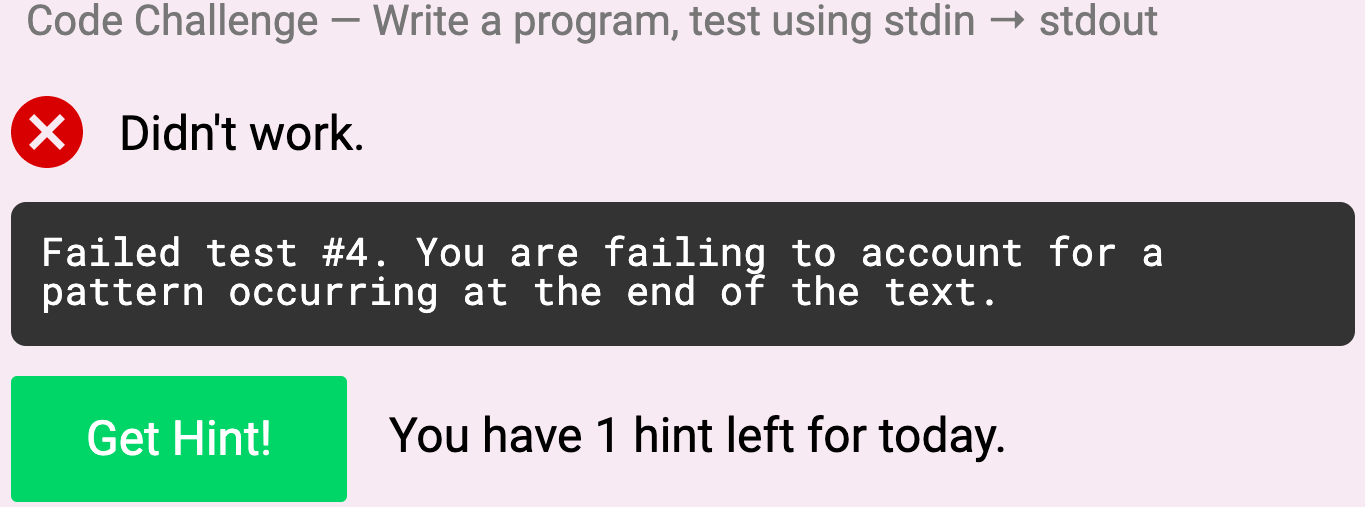
\includegraphics[width=0.85\textwidth]{figs/education-code-challenge-feedback}\\
(c)\\
\caption[Example Code Challenge]
{Example code challenge. (a) Each problem has a clear prompt, and (b) students can solve the problems directly within the text. In this example solution, the student has an off-by-one bug (the student misses the last index), and (c) the carefully-designed \gls{ITS} is able to provide the student personalized feedback.}
\label{fig:education-code-challenge}
\end{figure}

\subsubsection{Inquiry-Based Learning}
In introductory computational courses, the topics that are covered are rarely very interesting when presented out-of-context. When I present new topics in my \glspl{MAIT}, I first motivate them using a real-world problem in the form of a story. By employing Inquiry-Based Learning, an educational strategy in which students perform tasks in a fashion similar to those undertaken by professional scientists in order to construct knowledge~\cite{Pedaste2015}.

\subsubsection{Discovery Learning}
Research into Discovery Learning has showed that, when a student finds the solution to an open-ended problem on their own, the student benefits two-fold: the student typically has a stronger fundamental understanding of the solution, and the student has an improved perception of his or her own abilities to solve problems of this nature~\cite{Bruner1961}. In my \glspl{MAIT}, instead of simply presenting the learning goal to the student, I try to \textit{guide} the students and have them discover the solution on their own.

\subsubsection{Making Learning Fun!}
In my own experiences as a student, I often found it difficult to complete assigned reading assignments and would quickly lose interest during classes. In computational textbooks and learning resources, I often felt as though the learning materials were presented in a manner that was unneededly dry and complex. Instead, I fill my \glspl{MAIT} with stories, jokes, and puns, and I attempt to avoid the use of unnecessarily complex jargon when describing concepts to ensure that students of a wide range of backgrounds are able to follow successfully. I feel as though the success to learning is in the hands of the \textit{learners}, and it is the responsibility of the teacher as the expert to design the educational journey to be genuinely captivating. Intuitively, it is much easier to teach when students \textit{want} to learn.

\section{Results}
\subsection{Analyze Your Genome!}
TODO

\subsection{Data Structures}
TODO

\section{Discussion}
TALK ABOUT THE BROADER IMPACTS, E.G. ADOPTION BY PROFESSORS, IMPROVING AVAILABILITY, ETC.

%% END EDUCATION CHAPTER